\question[10] En la Figura \ref{fig:sucesion_triangulos01} se construye cada diseño con triángulos, añadiendo palillos de la
siguiente manera.

\begin{figure}[H]
    \centering
    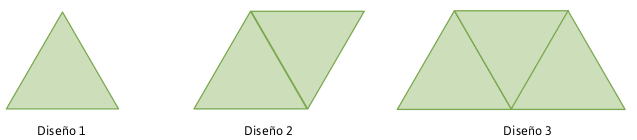
\includegraphics[width=.6\linewidth]{../images/sucesion_triangulos01}
    \caption{}
    \label{fig:sucesion_triangulos01}
\end{figure}

\begin{parts}
    \part Escribe una regla para la sucesión del número de palillos y compruébala.
    \part Reúnanse en equipo. Comprueben si obtuvieron una fórmula igual o equivalente a partir de sus resultados. En caso necesario, corrijan y argumenten por qué.
    \part Calculen cuántos palillos se tienen en total en el diseño 19.
    \part Toma en cuenta las reglas $20 + n$ y $13 + 2(n - 6)$ y calculen su valor para n = 19.
    \part Comparen los resultados de los incisos c) y d). ¿Cómo son? ¿Por qué?
    \part Basados en los valores de la regla que cada uno encontró y de estas dos, ¿las ex-
    presiones son equivalentes? Expliquen.
\end{parts}